\documentclass[10pt,a4paper,final]{scrartcl}
\usepackage[utf8]{inputenc}
\usepackage{amsmath}
\usepackage{amsfonts}
\usepackage{amssymb}
\usepackage{graphicx}
\usepackage{caption}
\usepackage{subcaption}
\usepackage{float}
\usepackage{endnotes}
\makeatletter
\def\enoteheading{\section{References
  \@mkboth{\MakeUppercase{\notesname}}{\MakeUppercase{\notesname}}}%
  \mbox{}\par\vskip-2.3\baselineskip\noindent\rule{.5\textwidth}{0.4pt}\par\vskip\baselineskip}
\makeatother

\author{
Group No.: 05 \\ 
Group Members: \\
LIU Xinhong (53043714) \\
LI Tong (53043505) \\
ZHONG Yuqing (53057522)
}
\titlehead{
City University of Hong Kong \\
Department of Electronic Engineering
}
\title{
EE3316 Information Product Design \\ Mobile App Design Final Report \\ Into Heart}
\subtitle{2013/14 (Semester B)}
\begin{document}
\maketitle

\pagebreak

\begin{abstract}
Heart is a vital organ of human body, once it stops, no matter how strong, you are gone.  
This app monitors heart rate all-day and evaluate heart health condition, integrates into everyday exercise training session and help user to control the exercise strength, to reach a better exercise goal, as well as training heart. With social integration, this app connects user with friends and family to motivate user care about their heart. This app also conducts emergency alert including: contacting the family, call ambulance, make noise, or any other viable first aids. 
\end{abstract}



\tableofcontents

\section{Introduction}

\subsection{Market Research}
Cardiovascular diseases (CVDs) are a group of disorders of the heart and blood vessel. In 2012 it kills 17 million people, makes 31\% of all death in the world\endnote{WHO, Cardiovascular diseases (CVDs), retrieved from http://www.who.int/mediacentre/factsheets\\/fs317/en/ on Feb 2, 2015 }. 
According to some researches, heart rate (HR) is an independent predictor of cardiovascular and all-cause mortality in men and women with and without diagnosed cardiovascular disease.\endnote{Kim Fox, MD, (2007) FESC, Resting Heart Rate in Cardiovascular Disease, Journal of the American College of Cardiology} Heart rate was assigned the same weighting as blood pressure and cardiorespiratory fitness in the overall score. On the other hand, It's vital to monitor your heart rate during exercise. A target heart rate is recommended to reach best exercise goal. Time is important when heart attack suddenly occur, time is life, handling emergency situation is a problem when patient is not near there relatives. 


\subsection{App Summary}
\subsubsection{Target User Group}
This App applies to almost all the people who care for their heart health. For those who suffer from heart disease, this App is a great tool to improve their heart condition and even save their lives. 
\subsubsection{Competitive Analysis}

The possible competitors in Android market are Instant Heart Rate, Runtastic Heart Rate,Heart Rate Monitor, Cardiograph, Up by Jawbone and Polar Beat. The most common method of these Apps to measure heart rate is as such: let the user put their finger on phone camera and at the same time turn on the flashlight. Usually the whole measurement will finish within one minute. The most popular one Instant Heart Rate is downloaded over ten million times. While they have few functions except for measuring heart rate. Up by Jawbone and Polar Beat use external sensor, which improve the accuracy, but their function mainly focuses on diet control or exercise record.  In comparison, our App uses an additional sensor to measure the heart rate so that it can automatically respond to user's heart condition at any time.In addition, our app also helps user to control their exercise life, adjust energy expenditure. And we also have the life style record function to monitor the user's bad habbits.Moreover, we add an additional function-emergency calling-to help users reduce the risk of lacking timely treatment.From this point of view, our App is innovative enough to compete in the market.  

\subsubsection{Target Platforms and Device Configurations}
\begin{tabular}{|c|c|}
\hline 
Item & Description \\ 
\hline 
Target platform & Android 4.3 or later \\
Networking & required if want to use social function \\
Screen resolution & no restriction \\
Touch screen & required \\
Processor & mainstream is fine \\
Bluetooth & required, LE preferred \\
Accessory & Polar™ H7 Heart Rate Sensor \\
\hline 
\end{tabular} 
\section{App Design and Analysis}
\subsection{User Scenarios}
	Our app has free entry for all. It would feedback the heart rate immediately and also exercise information to ordinary user when the external connection was built, such as Millet bracelet. Evaluation report is provided. An additional function is designed for persons who have diseases related to heart, when the system detects your heart rate abnormal, it would call the people whom you set before automatically to save you. Some optional function such as login, comparison with friends would also be attached in this app to encourage user to be healthier. 
 
Our app aims to give people a chance to pay attention to them healthy condition, and also offer seasonable assistance to their daily life. It is expected to be practical in helping people. The comparison session is supposed to motivate person to improve their healthy condition. The UI would be simple and useful, which makes user feel convenient to use this app. 
\subsection{Screen and Interactivity Design}
	\begin{figure}
\centering
\begin{subfigure}{.24\textwidth}
  \centering
  \includegraphics[width=.8\linewidth]{img/screenshot/ss1-eps-converted-to.pdf}
  \caption{Dashboard}
\end{subfigure}%
\begin{subfigure}{.24\textwidth}
  \centering
  \includegraphics[width=.8\linewidth]{img/screenshot/ss2-eps-converted-to.pdf}
  \caption{Rating smoking}
\end{subfigure}
\begin{subfigure}{.24\textwidth}
  \centering
  \includegraphics[width=.8\linewidth]{img/screenshot/ss3-eps-converted-to.pdf}
  \caption{Search friend}
\end{subfigure}
\begin{subfigure}{.24\textwidth}
  \centering
  \includegraphics[width=.8\linewidth]{img/screenshot/ss4-eps-converted-to.pdf}
  \caption{Analysis}
\end{subfigure}
\begin{subfigure}{.24\textwidth}
  \centering
  \includegraphics[width=.8\linewidth]{img/screenshot/ss5-eps-converted-to.pdf}
  \caption{User info}
\end{subfigure}%
\begin{subfigure}{.24\textwidth}
  \centering
  \includegraphics[width=.8\linewidth]{img/screenshot/ss6-eps-converted-to.pdf}
  \caption{Calling}
\end{subfigure}
\begin{subfigure}{.24\textwidth}
  \centering
  \includegraphics[width=.8\linewidth]{img/screenshot/ss12-eps-converted-to.pdf}
  \caption{Disease Pedia}
\end{subfigure}
\begin{subfigure}{.24\textwidth}
  \centering
  \includegraphics[width=.8\linewidth]{img/screenshot/ss7-eps-converted-to.pdf}
  \caption{Exercise mode}
\end{subfigure}
\begin{subfigure}{.24\textwidth}
  \centering
  \includegraphics[width=.8\linewidth]{img/screenshot/ss8-eps-converted-to.pdf}
  \caption{Ranking}
\end{subfigure}%
\begin{subfigure}{.24\textwidth}
  \centering
  \includegraphics[width=.8\linewidth]{img/screenshot/ss9-eps-converted-to.pdf}
  \caption{Life style}
\end{subfigure}
\begin{subfigure}{.24\textwidth}
  \centering
  \includegraphics[width=.8\linewidth]{img/screenshot/ss10-eps-converted-to.pdf}
  \caption{Open page}
\end{subfigure}
\begin{subfigure}{.24\textwidth}
  \centering
  \includegraphics[width=.8\linewidth]{img/screenshot/ss11-eps-converted-to.pdf}
  \caption{Navigation}
\end{subfigure}
\caption{Screenshots of Into Heart}
\label{fig:ss}
\end{figure}
See Figure \ref{fig:ss}.
\subsection{Functional Requirements}
	Based on your use cases, derive functions of your app that must be implemented to allow a user to perform the tasks. A function is described as a set of inputs, the behaviour, and outputs. 

\begin{itemize}

\item System shall show the start page then Dashboard(Normal Mode). \textless User open the "Into Heart" app\textgreater
\item System shall show the navigation menu. \textless User press the menu button or slides to right\textgreater 
\item System shall let user allow the Bluetooth and connect to the sensor. \textless User press "Sensor" in menu\textgreater 
\item System shall show the user information and could modify them. \textless User press the "My info" in menu and press "Save" button\textgreater 
\item System shall let user input username, E-mail, password to create a new account. \textless User press "Create An Account" in "My info"\textgreater 
\item System shall let user input E-mail and password and log in the account. \textless User press "Log in" in "My info"\textgreater 
\item System shall jump to user page where not logged in. \textless User press "Sign Out" in "My info"\textgreater 
\item System shall show heart rate diagram of instant, day, week, month respectively. \textless User press "Instant Heart Rate", "Day", "Week", "Month" in "Dashboard", respectively\textgreater 
\item System should show exercise mode and give an artificial voice reminder. \textless User press "Exercise Mode" on "Dashboard" when it is in "Normal Mode"\textgreater 
\item System should give a warning voice reminder or even call the emergency number. \textless User's heart rate is out of regular range\textgreater 
\item System shall show the setting window and user could toggle whether enable the emergency call. \textless User press setting button at right corner\textgreater 
\item System shall show average, minimum, maximum of recent heart rate, as well as predicted kind of heart disease. \textless User press "Analysis" in menu\textgreater 
\item System shall show popup window of diseases and could search for wikipedia. \textless User press "View tachycardia details" or "View bradycardia details" and enter into any diseases\textgreater 
\item System shall show ranking page, which calculates users' total \endnote{American Heart Association, retrieved from 
http://www.heart.org/HEARTORG/GettingHealthy/\\PhysicalActivity/FitnessBasics/Target-Heart-Rates\_UCM\_434341\_Article.jsp on Apr 10, 2015 }score and makes comparisons. \textless User press "Ranking" in menu\textgreater 
\item System shall show adding friend page and could search for new friends. \textless User press add friends button on "Ranking"\textgreater 
\item System shall show the life record page. \textless User press "Life Style" in menu\textgreater 
\item System shall popup windows to record life habit. \textless User press either five icons and change the rating bar\textgreater 

\end{itemize} 

\subsection{Non-Functional Requirements}
	No specific performance requirement, or other non-functional requirements need special attention.
\subsection{Architectural Design}
\begin{figure}[H]
\centering
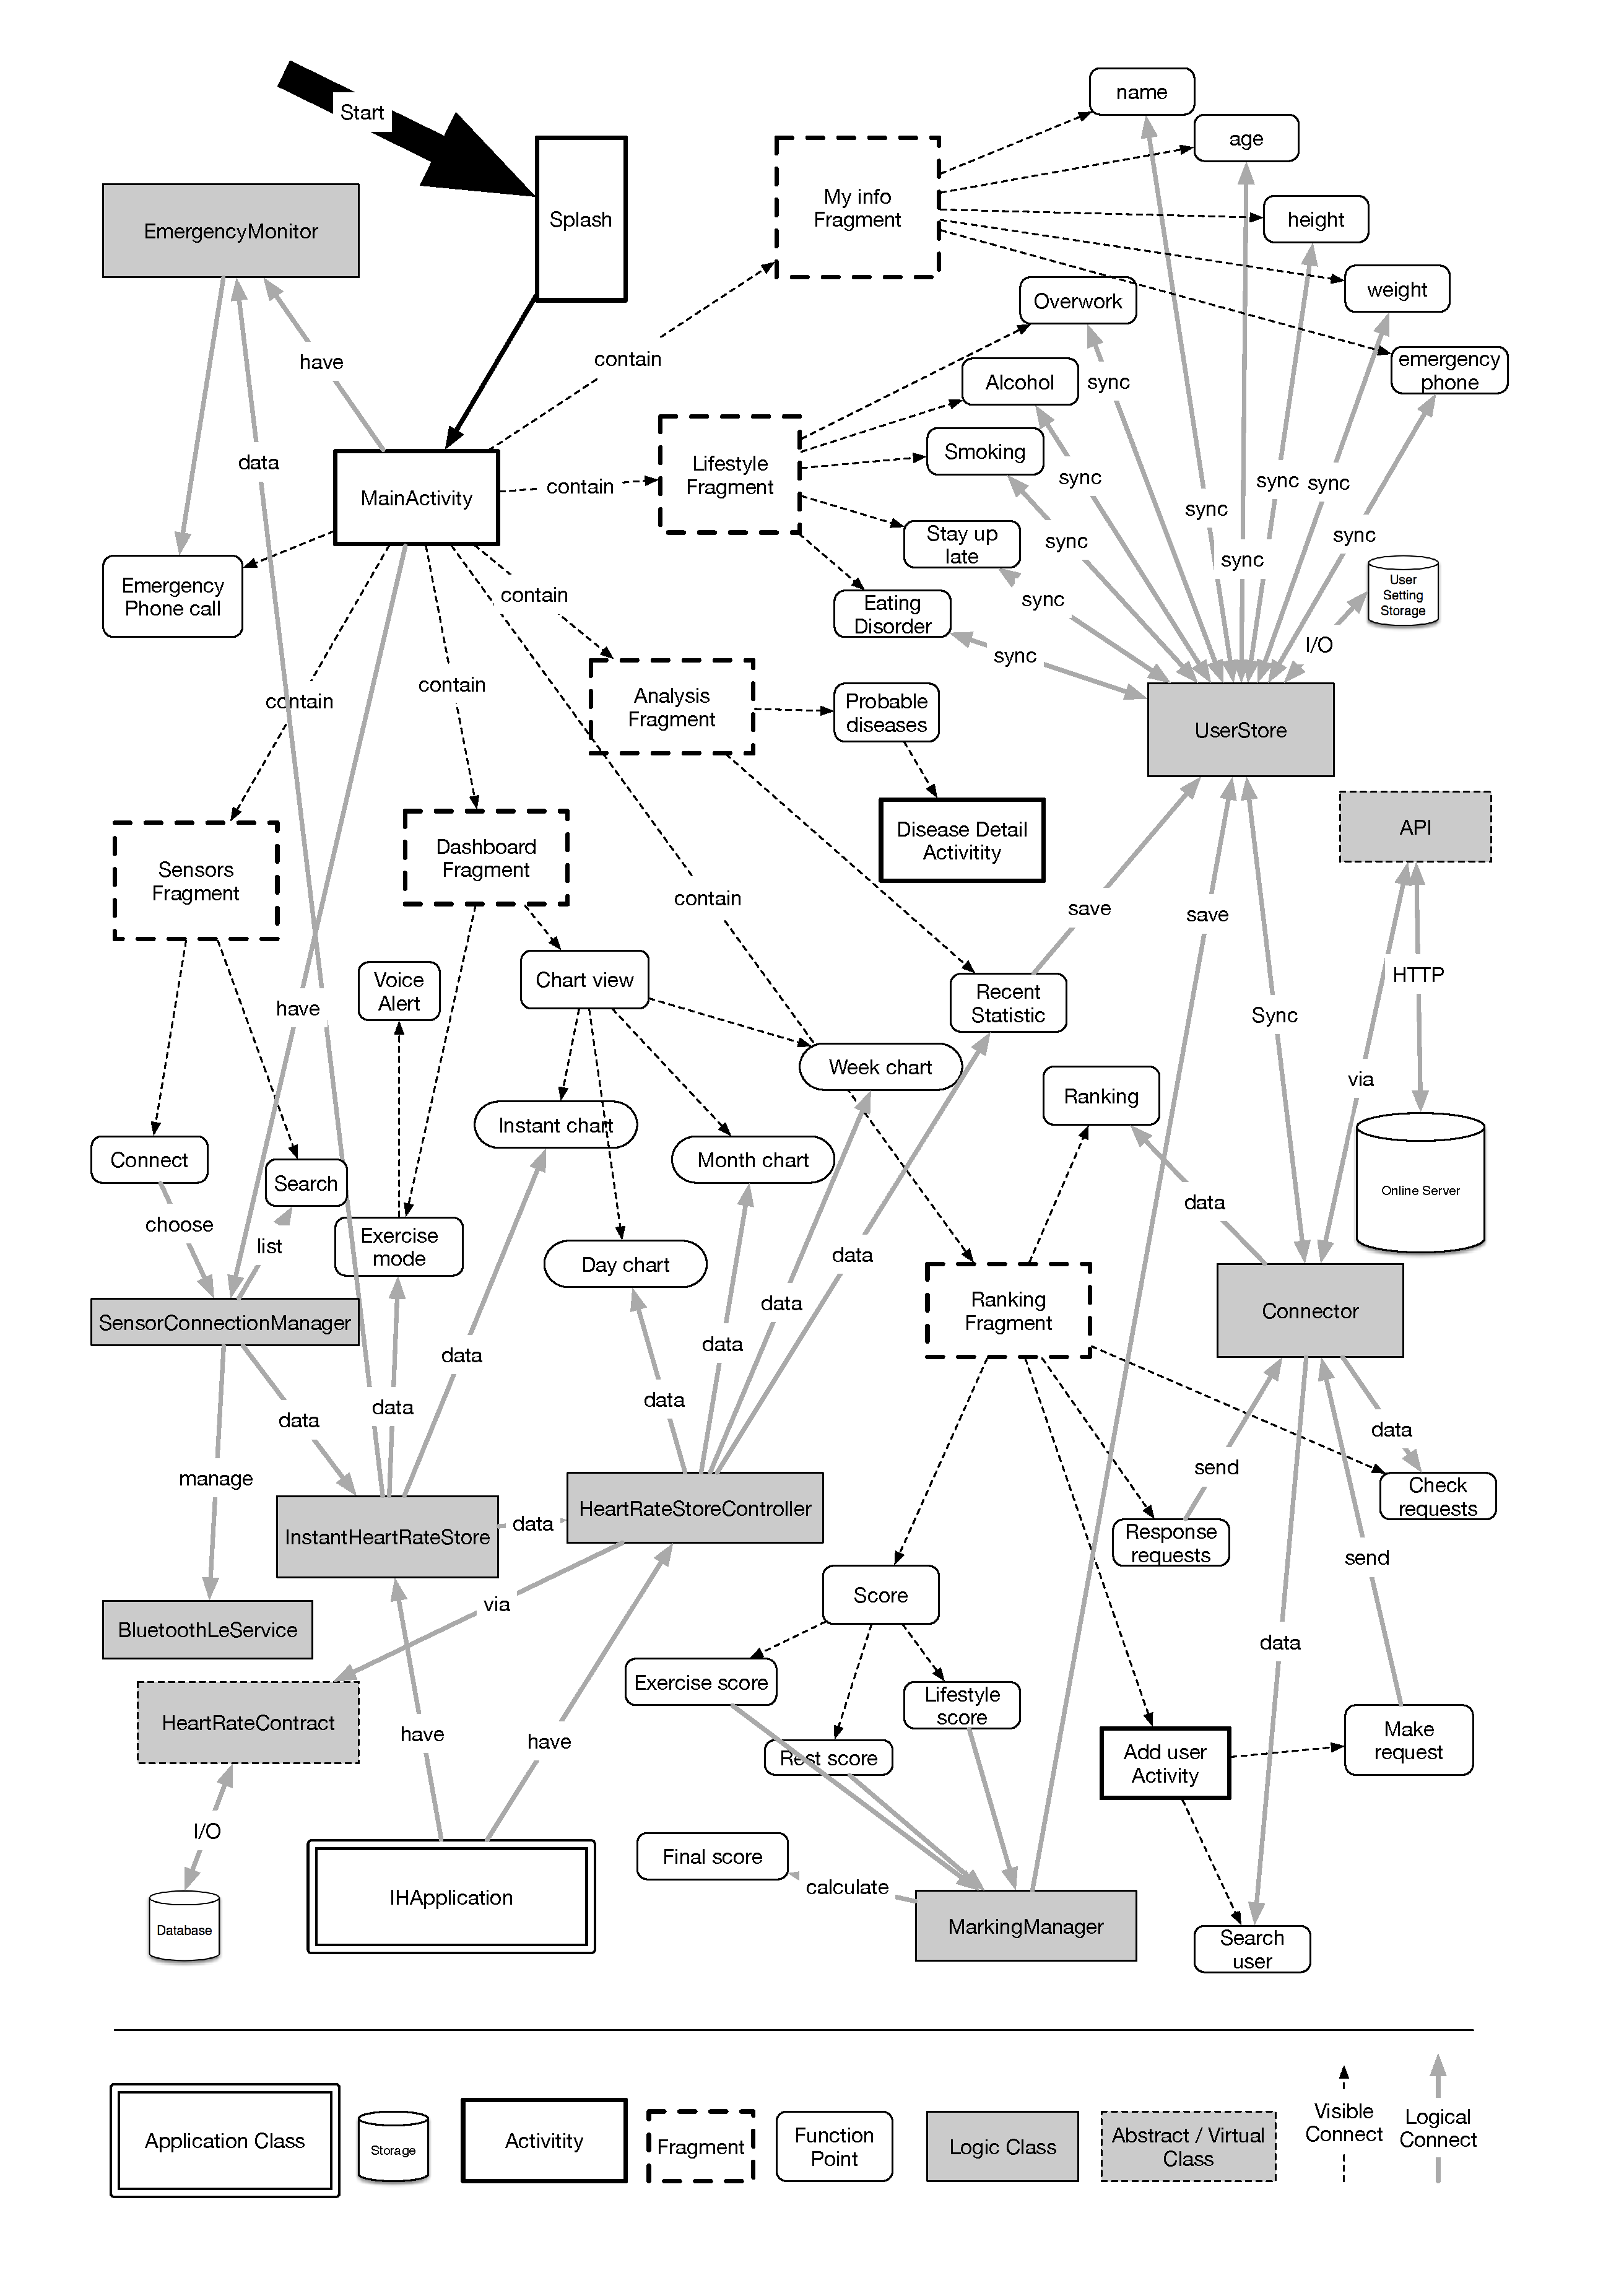
\includegraphics[width=5.3in]{img/arch.eps}
\caption{Into Heart Architectural Design}
\label{fig:arch}
\end{figure}

\section{Configuration}
\subsection{Configuration}
	\subsubsection{App}
For Into Heart App, we use Android Studio project structure with Gradle project automation tool to do package management. The project bone structure is as followed.

\paragraph{IHApplication.java} is the Application class and holds global variables.
\paragraph{MainActivity.java} is the main activity with a navigation drawer to navigate between fragments, also the inner class EmergencyMonitor monitor heart rate and make emergency call when necessary.
\subparagraph{NavigationDrawerFragment.java} is navigation drawer fragment, let user navigate between fragments.
\subparagraph{DashboardFragment.java} is under MainActivity and let users view the instant heart rate and historical charts, as well as exercise mode.
\subparagraph{AnalysisFragment.java} is under MainActivity and let users view their recent heart rate analysis result  and the diseases they might have.
\subparagraph{SensorsFragment.java} is under MainActivity and let users search the sensors nearby and connect to them.
\subparagraph{RankingFragment.java} is under MainActivity and let user view their score and the ranking among friends. Searching friends, sending friend requests and responding the requests are in this fragment.
\subparagraph{UserInfoFragment.java} is under MainActivity and let user set their basic informations such as name, age, weight, height and emergency telephone.
\subparagraph{LifestyleFragment.java} is under MainActivity and let user rate their lifestyle, including smoking, alcohol, eating disorder, stay up late and overwork.
\paragraph{AddFriendActivity.java} can be entered from RankingFragment, letting user search and send friend request.
\paragraph{RawDataActivity.java} let user view the raw data of data tale "day"
\paragraph{SettingsActivity.java} responds the interaction when user clicks on the setting page.
\paragraph{Splash.java} Splash page.
\paragraph{DiseaseDetailActivity.java} shows the detail of a particular disease using a WebView.
\paragraph{UIComponent/SimpleAlertController.java} is just a wrapper of AlertDialog, for easier usage.
\paragraph{HTTP/API.java} defines the communication prototype between app and server.
\paragraph{HTTP/Connector.java} defines the methods to use API to communicate with server.
\paragraph{HTTP/JCallback.java} is just a wrapper for handler, for easier asynchronous programming especially in networking.
\paragraph{HTTP/Outcome} is the Data model passing in JCallback.
\paragraph{Data/HeartRateContract.java} defines the database model and some simple query/insert methods.
\paragraph{Data/HeartRateStoreController.java} controls all data coming in/out the database.
\paragraph{Data/InstantHeartRateStore.java} stores the recent 60 heart rate data from sensors.
\paragraph{Data/MarkingManager.java} defines the rules of marking scores.
\paragraph{Data/UserStore.java} is the controller to control the user's info and scores, sync the data with server using Connector and sync the data locally using {\bf SharedPreferences}.
\paragraph{BLE/BluetoothLeService.java} is registered service to communicate with Bluetooth LE device.
\paragraph{BLE/GattAttributes.java} stores some constants conforms to Generic Attribute Profile.
\paragraph{BLE/SensorConnectionManager.java} manages the connections between sensor and app, also handle the data sent from sensor and pass to other objects.


\paragraph{res/layout/*} are the layout files defines the static layouts used by activities, fragments, alert dialogs and lists.
\paragraph{res/menu/*} define the action menu bar's items.
\paragraph{res/drawables-*/* and res/minmap-*/*} are image resources.
\paragraph{res/values/*} define the string constants and other static resources.
\paragraph{res/xml/*} define the setting items.





\subsubsection{Server}

Since the stress is not on the server side, only the basic configurations are mentioned below.

For rapidly development, our server-side choice is to use Ubuntu 14.04 server version as OS, with node.js server application, express framework and MongoDB database system. 

\paragraph{routes/users.js} handles all requests with endpoints /users/*.
\paragraph{models/models.js} defines the data models.
\paragraph{app.js} initialize and starts the application, making connection with database.

\subsection{Known Issues}
	\paragraph{Crash when switching fragment while networking work not finished.} 
When networking is still on, quickly switch fragment cause fragment dettached, then "getActivity()" will return null which further cause crash of the app. Some optimization like null checking is added, the bug emerges less. 
\paragraph{Old version of lifestyles or other settings takes place of right version when network condition is not well.}
There exists a case where the fetching from server starts, user modifies the lifestyle rating, and the modified data is transferred to server, at this time or then, the previous fetching finished, the old lifestyles overwrite the local ones, and when user does changes based on this old version, it will misleads the e data is not synced. This bug is being fixed and emerges sometimes. 
\paragraph{TTS fails to get the speaking status.}
In exercise mode, the speaking status cannot be got which would be used for preventing voice from erupting at same time. Currently fallback is let TTS not receiving any request for 10 seconds after each request, or called "cool down period". 
\paragraph{Not be able to keep exercise mode.}
When in exercise mode, if user change to other pages by navigation menu, after coming back to "Dashboard", the mode turns back to normal mode, but not remains on the exercise mode. 
\paragraph{Exercise mode backs to Normal mode when switch out the dashboard then back.} This is because the exercise mode is hosted in dashboard fragment, currently the best solution is to move the entire related code to the activity, while there is a lot work to do and no time for this.

\subsection{User Manual}
	\begin{enumerate}
\item Press "Into Heart" icon to launch the application 
\item After the open page, you could see the menu and "Dashboard", choose "Sensor" in menu and wear the H7 sensor. If your are asked to turn on the Bluetooth, choose "Allow". Build the connection between your device and the sensor. 
\item Go to "My info" page to create account if it is your first time to use this app, then log in by pressing the "Log in" button. You could modify your age, height, weight as well as emergency number, and save.  
\item More functions: 
\begin{itemize}
\item Save your life: In the "Dashboard", your heart rate could be detected and shown in day, week, and month. On the right corner, you could change the mode between "Normal Mode" and "Exercise Mode". If your heart rate is irregular, the system would automatically call to your emergency number to save your life! Exercise mode would give you an artificial voice reminder. 
\item Analysis: This page will show your average, maximum, minimum heart rate and give you an analytical result of your health condition. Press "View details", then you can see a WikiPedia list about different heart diseases.  
\item Sharing with friends: If you has logged in, you could see your health score and ranking between your friends in "Ranking" page, press the add friend button you could also search for and add new friends. 
\item Record: In the "Life Style" page, you can press on either icon to set your life habits. 
\end{itemize}
\end{enumerate}

\section{Conclusion}
\subsection{Evaluation}
	\paragraph{Conclusion of work}
There are 3 members in our group. Li Tong and Zhong Yuqing are responsible for UI design. Which also includes implementing UI design into xml activity format, linking UI and collect bugs reported from tester. Liu Xinhong is responsible for the app logic, class design and class implementation. Testing is conducted by all members.  All of us are conscientious and good at cooperating. 
                                
\paragraph{Comment on the result and completion level}
After all the developments, our app is complicated and contains a great number of functions, which is coincident with our original planning ideas. For instance, we discussed about the functions like emergency calling, artificial voice reminder, adding friends and measuring the instant heart rate, etc. Such functions are all implemented successfully. Although there are still some issues we cannot resolve well in the end,  they somehow do not affect much to our app. By the way, we didn’t put up our app on the “Google Play” because it needs an external device which would not be owned by most of the users.  
 
\paragraph{Feedbacks}
We have shown our app to our classmates, friends and relatives. Some people think our app is fairly good and user friendly, and they like the style of our user interface; some consider our app as a useful heath assistant which reminds them to pay attention to their heart conditions; some students regard the sensor as an accurate mearusing tool while others think it is a little expensive and may not want to afford it. In addition, there are also some advises like we should add more attributes to predict the heart diseases, not only the heart rate. It would be better to improve the ranking page, for example, add a function to view the detail scores of our friends. 

All in all, we are pretty satisfied with our achievement, as well as how valuable experience we had gained from the process of developing “IntoHeart”. 


\theendnotes
 

\end{document}